\documentclass[landscape]{beamer}

\mode<handout>
    {
    \usepackage{pgf}
    \usepackage{pgfpages}

    \pgfpagesdeclarelayout{6 on 1 boxed}
    {
        \edef\pgfpageoptionheight{\the\paperheight}
        \edef\pgfpageoptionwidth{\the\paperwidth}
        \edef\pgfpageoptionborder{0pt}
    }
    {
        \pgfpagesphysicalpageoptions
        {%
            logical pages=6,%
            physical height=\pgfpageoptionheight,%
            physical width=\pgfpageoptionwidth%
        }
        \pgfpageslogicalpageoptions{1}
        {%
            border code=\pgfsetlinewidth{2pt}\pgfstroke,%
            border shrink=\pgfpageoptionborder,%
            resized width=.5\pgfphysicalwidth,%
            resized height=.5\pgfphysicalheight,%
            center=\pgfpoint{.25\pgfphysicalwidth}{.833\pgfphysicalheight}%
        }%
        \pgfpageslogicalpageoptions{2}
        {%
            border code=\pgfsetlinewidth{2pt}\pgfstroke,%
            border shrink=\pgfpageoptionborder,%
            resized width=.5\pgfphysicalwidth,%
            resized height=.5\pgfphysicalheight,%
            center=\pgfpoint{.75\pgfphysicalwidth}{.833\pgfphysicalheight}%
        }%
        \pgfpageslogicalpageoptions{3}
        {%
            border code=\pgfsetlinewidth{2pt}\pgfstroke,%
            border shrink=\pgfpageoptionborder,%
            resized width=.5\pgfphysicalwidth,%
            resized height=.5\pgfphysicalheight,%
            center=\pgfpoint{.25\pgfphysicalwidth}{.5\pgfphysicalheight}%
        }%
        \pgfpageslogicalpageoptions{4}
        {%
            border code=\pgfsetlinewidth{2pt}\pgfstroke,%
            border shrink=\pgfpageoptionborder,%
            resized width=.5\pgfphysicalwidth,%
            resized height=.5\pgfphysicalheight,%
            center=\pgfpoint{.75\pgfphysicalwidth}{.5\pgfphysicalheight}%
        }%
        \pgfpageslogicalpageoptions{5}
        {%
            border code=\pgfsetlinewidth{2pt}\pgfstroke,%
            border shrink=\pgfpageoptionborder,%
            resized width=.5\pgfphysicalwidth,%
            resized height=.5\pgfphysicalheight,%
            center=\pgfpoint{.25\pgfphysicalwidth}{.167\pgfphysicalheight}%
        }%
        \pgfpageslogicalpageoptions{6}
        {%
            border code=\pgfsetlinewidth{2pt}\pgfstroke,%
            border shrink=\pgfpageoptionborder,%
            resized width=.5\pgfphysicalwidth,%
            resized height=.5\pgfphysicalheight,%
            center=\pgfpoint{.75\pgfphysicalwidth}{.167\pgfphysicalheight}%
        }%
    }


    \pgfpagesuselayout{6 on 1 boxed}[letterpaper, border shrink=5mm]
    \nofiles
}

%\usetheme{Antibes}
%\usetheme[compress]{Singapore}
\usetheme{Warsaw}
\usecolortheme{seahorse}

\hypersetup{pdfpagemode=FullScreen}

%\definecolor{amber}{rgb}{1.0, 0.75, 0.0}
%\definecolor{alizarin}{rgb}{0.39, 0.58, 0.93}
%\setbeamercolor{structure}{fg=amber!85!black}
\usefonttheme[onlymath]{serif}
%\setbeamercovered{transparent}

\usepackage[T1]{fontenc}
\usepackage{colortbl}
\usepackage{multimedia}
\usepackage{graphicx}
\usepackage{lmodern, textcomp}
\usepackage{multicol}
\setlength{\columnsep}{1cm}
\usepackage{xcolor}
\usepackage{tikz,tkz-euclide}
\usetikzlibrary{calc}
\usetikzlibrary{decorations.pathreplacing}
\usetikzlibrary{shapes.misc, positioning}
\tikzset{vertex/.style={circle, fill=black, draw=black, inner sep=0pt, minimum size=1.15ex}}
%%%%%%%%%%%%%%%%%%%%%%%%%%%%%%%%%%%%%%%%

\usepackage{graphicx}  % Required for including images
\graphicspath{{./images/}}

\newcommand{\Z}{\ensuremath{Z}}
\newcommand{\K}[1][3]{\ensuremath{K^{(#1)}}}
\let\Lstroke=\L
\renewcommand{\L}[1][3]{\ensuremath{L^{(#1)}}}
\newcommand\multiset[2][\lambda]{\vphantom{#2}^{#1\!}#2}
\let\ms=\multiset

\newtheorem{maintheorem}{Main Theorem}

\definecolor{darkgreen}{rgb}{0,0.39,0}
\definecolor{darkred}{rgb}{0.5,0.1,0.1}
%\colorlet{mygold}{amber!85!black}

\newcommand\drawHedge[4][]{\draw [thick, #1] (#2) edge[bend left] (#3) edge (#4) (#3) edge (#4);}
%%%%%%%%%%%%%%%%%%%%%%%%%%%%%%%%%%%%%%%%

\title[Grates]{``Grate'' Expectations}

%\author[Fields and Darrow] {Joe Fields and Brian~Darrow,~Jr.\texorpdfstring{\rlap,}*\\
%\vspace{1em}
%Southern Connecticut State University}
\author[Darrow] {Brian~Darrow,~Jr., Ph.D.}
\institute[SCSU]{Central Connecticut State University\\}
% \medskip
% (Joint work with Joe Fields)}

\date[CCSU Spring 2025] {Mathematics Department Colloquium \\[1em]
\small Central Connecticut State University \\
\small New Britain, CT\\
\small February 21, 2025}

% \newcommand\grantNumber{A1950357}
% \newcommand\grantTitle{REU\slash RET Site: Mathematics Research Experience \\ for Pre-Service and for In-Service Teachers}


%%%%%%%%%%%%%%%%%%%%%%%%%%%%%%%%%%%%%%%%

\begin{document}

    \maketitle


    \section{Introduction}

%\subsection{Graph Decomposition}

    \begin{frame}{Abstract}

        \small{Originally inspired by the process of recording student grades on a traditional grade sheet, we define an $(n,k)$-grate to be a binary $n$-tuple containing $k$ ones, such that there are never two adjacent zeroes. After developing a formula to count the number of grates in terms of the parameters $n$ and $k$ (for which there is a pleasing combinatorial proof), we then consider the process of flipping the bits ($0$’s turning into $1$’s) of a sequence of $n$ zeroes until a grate is created. For a given value of $n$, we are interested in the expected number of bit-flips needed to obtain a grate. Hence, we obtain the fitting pun given in the title of the talk. (Rest assured, additional puns will be littered throughout the presentation!)\\

        \medskip

        In a talk aimed to be (mostly) accessible and interesting to mathematics majors and faculty alike, the many connections this problem has with famous mathematical work (e.g., Pascal's Triangle and the Fibonacci Sequence) will also be explored.}

    \end{frame}

        { %magic to get a full screen image...
        \setbeamertemplate{navigation symbols}{}  % hide navigation buttons
        \setbeamertemplate{background canvas}{\centerline{\includegraphics
        [height=\paperheight]{grade_sheet.JPG}}}
        \begin{frame}{Ever Been in this Situation?}
            \rule{0pt}{0pt}
        \end{frame}

    } %end of magic


        { %magic to get a full screen image...
        \setbeamertemplate{navigation symbols}{}  % hide navigation buttons
        \setbeamertemplate{background canvas}{\centerline{\includegraphics
        [height=\paperheight]{actual_grate.JPG}}}
        \begin{frame}[plain]
            \rule{0pt}{0pt}
        \end{frame}

    } %end of magic


    \begin{frame}{Grate Expectations}
        \begin{center}
            \includegraphics[scale=2]{DickensCover.pdf}
        \end{center}
    \end{frame}


    \begin{frame}{Grate Expectations}
        \transfade
        \begin{center}
            \includegraphics[scale=2]{DickensCover_Grate_2.jpg}
        \end{center}
    \end{frame}


    \begin{frame}{Grate Beginnings}
        \begin{itemize} \addtolength\itemsep{1em}
        \item My colleague Joe Fields (SCSU) first encountered the problem years ago while recording grades
        \item Fields shared the problem with me when I joined the faculty at Southern
        \item What has ensued has represented a microcosm of the mathematical endeavor, and what mathematics is all about
        \end{itemize}
    \end{frame}


    \begin{frame}{The Grate Problem}
        \begin{itemize} \addtolength\itemsep{1em}
        \item In recording scores by hand, a great deal of care is needed--until it's not.
        \item It's not, when you've entered enough grades so that only isolated cells, blank positions with no other blank positions adjacent to them, remain.
        \item We refer to such an arrangement as a \textit{grate}.
        \end{itemize}
    \end{frame}

    \begin{frame}{The Grate Problem}
        \begin{itemize} \addtolength\itemsep{1em}
        \item The problem that emerged is: What is the expected number of scores recorded before we will have a grate?
        \item There are some trivial bounds on this expected value.
        \end{itemize}
    \end{frame}

    \begin{frame}{Some Grate Bounds}
        \begin{itemize} \addtolength\itemsep{1em}
        \item If $n-1$ scores have been recorded, you certainly have a grate!
        \item If $n-2$ scores have been recorded, you \textit{usually} have a grate.
        \item If fewer than $\lfloor\frac{n}{2}\rfloor$ scores have been recorded, you certainly do not have a grate.
        \end{itemize}
    \end{frame}

    \section{First Steps}

    \begin{frame}{Grate Abstractions}
        \begin{itemize} \addtolength\itemsep{1em}
        \item Consider a permutation $\pi$ of $\{1, 2, 3, \ldots , n\}$.
        \item Beginning with a vector of length $n$ consisting of all $0$s, consider the following $n$-step procedure: For $i$ from $1$ to $n$ turn the zero in position $\pi(i)$ into a $1$.  A grate (in this context) is a binary vector having only isolated zeros.  Let $f(\pi)=k$ if at stage $k$ we have a grate but at stage $k-1$ we do not.  Assuming all permutations are equally likely, we have

        \[ E = \frac{1}{n!} \sum_{\pi \in S_n} f(\pi) \]
        \end{itemize}
    \end{frame}

    \begin{frame}{Some Grate Geometry}
        \begin{itemize} \addtolength\itemsep{1em}
        \item One way to think about this problem is to imagine the $n$-hypercube, with the origin $\vec{0}$ representing the all-zeroes vector, and $\vec{1}$ representing the all-ones vector.
        \item There are two parameters for a grate, the length $n$ and the number of ones, $k$ (which can be thought of as having weight $k$).
        \item We would then be concerned with the increasing paths from the bottom ($\vec{0}$) to the top ($\vec{1}$) of the $n$-hypercube (as a graded poset) which first encounter a grate at stage $k$, weighted by $k$.
        \item Of particular importance are what we call ``transition edges'', or those connecting a non-grate to a grate.
        \end{itemize}
    \end{frame}



    \begin{frame}{A Not-So-Grate Start}
        \begin{itemize} \addtolength\itemsep{1em}
        \item Without any idea of how to begin this problem, we naturally started finding the number of grates that exist for each pair of $n$ and $k$. \pause
        \item By brute force!
        \end{itemize}
    \end{frame}


    \begin{frame}{Grate Possibilities}
        \begin{table}[htbp]
            \begin{tabular}{|r||c|c|c|c|c|c|} \hline
            & $k=1$ & 2 & 3 & 4 & 5 & 6 \\ \hline\hline
            $n=1$   & 1     &       &       &       &       & \\[8pt] \hline
%
            $2$     & 10    & 11    &       &       &       & \\
            & 01    &       &       &       &       & \\[8pt] \hline
%
            $3$     & 010   &  011  & 111   &       &       & \\
            &       &  101  &       &       &       & \\
            &       &  110  &       &       &       & \\[8pt] \hline
%
            $4$     &       & 0101  & 0111  & 1111  &       & \\
            &       & 1010  & 1011  &       &       & \\
            &       & 0110  & 1101  &       &       & \\
            &       &       & 1110  &       &       & \\[8pt] \hline
            \end{tabular}
        \end{table}
    \end{frame}


    \begin{frame}{Grate Possibilities}
        \begin{table}[htbp]
            \begin{tabular}{|r||c|c|c|c|c|c|} \hline
            & $k=1$ & 2 & 3 & 4 & 5 & 6 \\ \hline\hline
            $5$     &       & 01010 & 01011 & 01111 & 11111 & \\
            &       &       & 10101 & 10111 &       & \\
            &       &       & 01101 & 11011 &       & \\
            &       &       & 01110 & 11101 &       & \\
            &       &       & 10110 & 11110 &       & \\
            &       &       & 11010 &       &       & \\[8pt] \hline
            \end{tabular}
        \end{table}
    \end{frame}

    \begin{frame}{Grate Possibilities}
        \begin{table}[htbp]
            \begin{tabular}{|r||c|c|c|c|c|c|} \hline
            & $k=1$ & 2 & 3 & 4 & 5 & 6 \\ \hline\hline
%
            $6$     &       &       & 010110& 010111 & 011111 & 111111 \\
            &       &       & 101010& 101011 & 101111 &       \\
            &       &       & 011010& 011011 & 110111 &       \\
            &       &       & 010101& 011101 & 111011 &        \\
            &       &       &       & 101101 & 111101 &        \\
            &       &       &       & 110101 & 111110 &       \\
            &       &       &       & 011110 &        & \\
            &       &       &       & 101110 &        & \\
            &       &       &       & 110110 &        & \\
            &       &       &       & 111010 &        & \\[8pt] \hline
            \end{tabular}
        \end{table}
    \end{frame}



    \begin{frame}{A Grate Recursion}
        \begin{itemize} \addtolength\itemsep{1em}
        \item We started by counting up the number of possible grates for small values of $n$ and $k$.\pause
        \item Eventually, we found a recursive approach to listing all the grates of a given length.\pause
        \item After too, too much time\dots\pause
        \item Of course! Pascal's Triangle!
        \end{itemize}
    \end{frame}



    \begin{frame}{The Grate Pascal's Triangle}
        \begin{table}[htbp]
            \begin{tabular}{|r||c|c|c|c|c|c|} \hline
            & $k=1$ & 2 & 3 & 4 & 5 & 6 \\ \hline\hline
            $n=1$  & 1    &      &       &       &       &   \\[8pt] \hline
            $2$     & 2   &  1   &       &       &       &   \\[8pt] \hline
            $3$     & 1   &  3   &   1   &       &       &   \\[8pt] \hline
            $4$     &     &  3   &   4   &    1  &       &   \\[8pt] \hline
            $5$     &     &  1   &   6   &    5  &     1 &   \\[8pt] \hline
            $6$     &     &      &   4   &   10  &     6 & 1 \\[8pt] \hline
            \end{tabular}
        \end{table}
    \end{frame}


    \begin{frame}{Our First Grate Conjecture}
        \begin{itemize} \addtolength\itemsep{1em}
        \item Let $g(n,k)$ denote the number of grates with length $n$ and $k$ ones. The recursion for binomial coefficients, and the shifting of the entries in Pascal's Triangle within the table, led us to conjecture that

        \[g(n,k)=g(n-1,k-1)+g(n-2,k-1)\]

        \item Note that $G(n,k)$ denotes the set of grates that exist for a given $n$ and $k$, while $g(n,k)=|G(n,k)|$
        \end{itemize}
    \end{frame}

% \begin{frame}{A Grate Example of the Recursion}
% \begin{itemize} \addtolength\itemsep{1em}
%   \item We will build the set $G(3,2)$ from the sets $G(2,1)$ and $G(1,1)$. Now, since $G(3-2,2-1)=G(1,1)=\{1\}$, we will append the string $10$ and yield $\{110\}$.\pause
%   \item Next, since $G(3-1,2-1)=G(2,1)=\{10,01\}$ to which we will append a single $1$, yielding the grates of $\{101,011\}$. Thus,

% \[ G(3,2)=\{110, 101,110\} \] \pause

% \noindent and \[g(3,2)=3\]

% \end{itemize}
% \end{frame}



    \begin{frame}{A Grate Example}
        \begin{table}[htbp]
            \begin{tabular}{|r||c|c|c|c|c|c|} \hline
            & $k=1$ & 2 & 3 & 4 & 5 & 6 \\ \hline\hline
            $n=1$   & 1     &       &       &       &       & \\[8pt] \hline
%
            $2$     & 10    & \cellcolor{green} 11    &       &       &       & \\
            & 01    &       &       &       &       & \\[8pt] \hline
%
            $3$     & 010   &  \cellcolor{yellow} 011  & 111   &       &       & \\
            &       &  \cellcolor{yellow}101  &       &       &       & \\
            &       &  \cellcolor{yellow}110  &       &       &       & \\[8pt] \hline
%
            $4$     &       & 0101  & \cellcolor{yellow}0111  & 1111  &       & \\
            &       & 1010  & \cellcolor{yellow}1011  &       &       & \\
            &       & 0110  & \cellcolor{yellow}1101  &       &       & \\
            &       &       & \cellcolor{green}1110  &       &       & \\[8pt] \hline
            \end{tabular}
        \end{table}
    \end{frame}

    \begin{frame}{Some Grate Notation, and a Grate Theorem}
        \begin{itemize} \addtolength\itemsep{1em}
        \item Let $f_b(v)$ denote the concatenation of the binary vector $v$ with a bitstring $b$. Thus, the operations we just described above are $f_1(v)$ and $f_{10}(v)$. We extend this function to apply to sets of vectors in the usual way

        \[f_b(S)=\{f_b(v) |  v\in S\}\]


        \begin{theorem}
            For $n\geq 2$ and $k\geq 1$,

            \[G(n,k)=f_{10}(G(n-2,k-1))\cup f_1(G(n-1,k-1))\]
        \end{theorem}

        \end{itemize}
    \end{frame}


    \begin{frame}{A Grate Proof!}
        \begin{itemize} \addtolength\itemsep{1em}
        \item First, $A = f_1(G(n-1,k-1))$ is a set of vectors that have length $n$ with $k$ ones. It's also clear that $B = f_{10}(G(n-2,k-1)$ is a set of vectors with length $n$ and $k$ ones.
        \item Note that the sets $A$ and $B$ are disjoint since $B$ consists solely of vectors that end with a 0, while $A$ consists entirely of vectors that end in with a $1$.
        \item  Further, note that the vectors in $A$ and $B$ contain only isolated zeros, so they are grates.  Thus $A \cup B \subseteq G(n,k)$.
        \end{itemize}
    \end{frame}


    \begin{frame}{A Grate Proof!}
        \begin{itemize} \addtolength\itemsep{1em}
        \item  To show the other inclusion, consider the final two bits in an element of $G(n,k)$, they can be $11$, $01$, or $10$ -- but not $00$, as that would violate the definition of a grate.
        \item  The first two possibilities end in a $1$, and with that $1$ deleted we would have an element of $G(n-1,k-1)$, so such vectors are in $A$.  Similarly, the grates that end in $10$, with those positions removed would lie in $G(n-2,k-1)$, so they are in $B$.
        \end{itemize}
    \end{frame}


    \begin{frame}{Another Grate Theorem}
        \begin{theorem}
            The number of bitstrings of length $n$ with $k$ 1s and only isolated 0s is $\binom{k+1}{n-k}$.
        \end{theorem}

    \end{frame}

    \begin{frame}{Another Grate Theorem and Proof }
        \begin{theorem}
            The number of bitstrings of length $n$ with $k$ 1s and only isolated 0s is $\binom{k+1}{n-k}$.
        \end{theorem}

        \begin{Proof}
            Consider a length $k$ bitstring containing all $1$'s.  There are $k+1$ positions before, after, or between these $1$'s. Then, select $n-k$ of those positions to insert the (individual) $0$'s.
        \end{Proof}

    \end{frame}




    \section{Expectation}

    \begin{frame}{Shifting the Focus to Grate Path Counting}
        \begin{itemize} \addtolength\itemsep{1em}
        \item Recall that we can think about this problem in terms of paths in the $n$-hypercube, $Q_n$.
        \item A ``path'' in $Q_n$ starts at $\vec{0}$, ends at $\vec{1}$, and always moving increasingly up the grade.
        \item All paths begin at a non-grate (unless $n=1$) and eventually pass into a grate.  Once a path has reached a node that is a grate, it will remain amongst the grates from that point onward.
        \item We're interested in counting the paths that first reach a grate after $k$ steps. In other words we want to count the paths that are at a non-grate at stage $k-1$ and hit a grate at stage $k$.
        \end{itemize}
    \end{frame}

    \begin{frame}{Shifting the Focus to Grate Path Counting}
        \begin{itemize} \addtolength\itemsep{1em}
        \item Consider the subgraph $G \leq Q_n$ consisting of nodes labelled by vectors of weight $k$ and $k-1$.  The nodes labelled by vectors of weight $k-1$ have degree $n-k+1$.
        \item The nodes labelled by vectors of weight $k$ have degree $k$.  Restricting our attention to the nodes of weight $k$ which are grates, we want to know how many edges are incident with them and a non-grate of weight $k-1$.
        \item Using our formula for the number of grates, and their degree in the subgraph $G$, we get a total number of incident edges -- from which we subtract the edges that are also incident with a grate of weight $k-1$.
        \end{itemize}
    \end{frame}

% \begin{frame}{A Grate Video, that's Not Embedded}
% Open Hypercube Video
% % \centering
% % \movie[label=show3,width=1.0\textwidth,poster
% %        ,autostart,showcontrols,loop]
% %   {movie}{HyperCube.mp4}
% \end{frame}


    \begin{frame}{Grate Permanence}
        \begin{itemize} \addtolength\itemsep{1em}
        \item Once you're a grate, you're always a grate
        \item This leads us to counting the edges that transition a non-grate to a grate
        \item Transition edges (going from level $k-1$ to level $k$):

        \[ \left[ k \binom{k+1}{n-k} - (n-k+1) \binom{k}{n-k+1} \right] \]

        \end{itemize}
    \end{frame}

    \begin{frame}{Grate Layers}
        \begin{center}
            \includegraphics[scale=.4]{GratePIC.PNG}
            % \input{grate_layers.pdf_t}
        \end{center}
    \end{frame}


    \begin{frame}{A Grate Result}
        \begin{itemize} \addtolength\itemsep{1em}
        \item Based on this, let $p(n,k)$ denote the number of paths in $Q_n$ that first encounter a grate after $k$ steps.  Since there are $(k-1)!$ ways to go from $\vec{0}$ to any vector of weight $k$, and there are $(n-k)!$ ways to proceed onward from a vector of weight $k$ to $\vec{1}$, we get

        \[ p(n,k) = \left[ k \binom{k+1}{n-k} - (n-k+1) \binom{k}{n-k+1} \right] \cdot (k-1)! \cdot (n-k)! \]

        \end{itemize}
    \end{frame}

    \begin{frame}{A Grate Result}
        \begin{itemize} \addtolength\itemsep{1em}
        \item A slightly more aesthetic form of
        \[ p(n,k) = \left[ k \binom{k+1}{n-k} - (n-k+1) \binom{k}{n-k+1} \right] \cdot (k-1)! \cdot (n-k)! \]
        is given by

        \[ p(n,k) = \left[ \binom{k+1}{n-k} - \binom{k-1}{n-k} \right] \cdot k! \cdot (n-k)! \]
        \end{itemize}
    \end{frame}







    \begin{frame}{Grate Expectations}
        \begin{itemize} \addtolength\itemsep{1em}
        \item From this, we get the formula for the expectation:

        \[ \frac{1}{n!} \cdot \sum_{k=1}^n k \cdot p(n,k). \]

        \item Taking note of the fact that $p(n,n) = 0$, and that $p(n,k) = 0$ whenever $k < \lfloor n/2 \rfloor$, this becomes

        \[ \frac{1}{n!} \cdot \sum_{k=\lfloor n/2 \rfloor}^{n-1} k \cdot \left[ \binom{k+1}{n-k} - \binom{k-1}{n-k} \right] \cdot (k)! \cdot (n-k)! \]

        \noindent
        \end{itemize}
    \end{frame}


    \begin{frame}{A Visually Grate Final Formula}
        \begin{itemize}
            \item Or in a more visually grate form (hence a separate slide)...
            \medskip
            \medskip

            \[\huge{\sum_{k=\lfloor n/2 \rfloor}^{n-1} k \cdot  \frac{\binom{k+1}{n-k} - \binom{k-1}{n-k}}{\binom{n}{k}} } \]

        \end{itemize}
    \end{frame}








    \begin{frame}{Is this Already a (Grate) Thing?}
        \begin{itemize} \addtolength\itemsep{1em}
        \item Throughout the duration of the project, we were concerned whether this problem had already been solved, perhaps under a different name
        \item As part of our due diligence, we searched the Online Encyclopedia of Integer Sequences for the sequence of numerators of our expected value
        \item After no results, we submitted our sequence, which was recently published (A365554) by N. J. A. Sloane himself! \cite{FieldsDarrow_OEIS}
        \end{itemize}
    \end{frame}


    \begin{frame}{First Pascal \dots Now Fibonacci?! How Grate!}
        \begin{itemize} \addtolength\itemsep{1em}
        \item The count of the transition edges is actually a sequence in OEIS,  A067331.
        \item The entry was ``Convolution of Fibonacci $F(n+1)$, $n\geq 0$, with $F(n+3)$, $n\geq 0$.''
        \item This was rather, let's say, ``unenlightening.''
        \item More investigation led to the discovery of Fibbinary numbers, which are just a bit-flip away from grates (not the expectation, however!)
        \end{itemize}
    \end{frame}

    \begin{frame}{First Pascal \dots Now Fibonacci?! How Grate!}
        \begin{itemize} \addtolength\itemsep{1em}
        \item It's well known that sums of the binomial coefficients in Pascal's triangle along lines of ``slope'' $\pm 1/2$ give Fibonacci numbers
        \item However, grates give us a nice combinatorial argument for this fact.
        \end{itemize}
    \end{frame}

    \begin{frame}{First Pascal \dots Now Fibonacci?! How Grate!}
        \begin{center}
            \includegraphics[scale=.30]{A-Pascals-Triangle-Fibonacci-Sequence-Mapping.png}
        \end{center}
% \cite{ResearchGate}
    \end{frame}



    \begin{frame}{First Pascal \dots Now Fibonacci?! How Grate!}
        \begin{theorem}
            $\displaystyle \forall n \in {\mathbb Z}^+, \; \sum_{k=\lfloor n/2 \rfloor}^n g(n,k) \; = \; F_{n+1}.$  Where $F_n$ denotes the $n$th Fibonacci number.
        \end{theorem}
    \end{frame}


    \begin{frame}{First Pascal \dots Now Fibonacci?! How Grate!}

        \begin{proof}
            Given any grate of length $n$, it either ends with a 0, or it doesn't.  If the final bit is a 1, we can delete it to obtain a grate of length $n-1$.  If the final bit is a 0, we can delete the last two positions, obtaining a grate of length $n-2$.  These processes are reversible.
            Thus, the number of grates of length $n$ satisfy the same recursion as the Fibonacci numbers. \\
            \medskip
            Adopting the convention that, at length $0$ there is a unique (vacuous) grate, and since there are two grates at length $n=1$, we have (except for an indexing offset) the same initial values as the Fibonacci numbers.
        \end{proof}
    \end{frame}




    \begin{frame}{A Deflating, Not-So-Grate Conclusion}
        \begin{itemize} \addtolength\itemsep{1em}
        \item In general, you will almost be done entering in your grades before your gradebook turns into a convenient grate!
        \end{itemize}
        \begin{table}[hbtp]
            \begin{tabular}{|r|c|c|} \hline
            $n$ & $E$  & $E/n$ \\ \hline \hline
            2 & 1.00 & 0.500 \\
            3 & 1.67 & 0.556 \\
            4 & 2.50 & 0.625 \\
            5 & 3.30 & 0.660 \\
            6 & 4.13 & 0.689 \\
            7 & 4.97 & 0.710 \\
            8 & 5.82 & 0.728 \\
            9 & 6.68 & 0.742 \\
            10 & 7.54 & 0.754 \\ \hline
            \end{tabular}
        \end{table}
    \end{frame}


    \begin{frame}{A Deflating, Not-So-Grate Conclusion}
        \begin{table}[hbtp]
            \begin{tabular}{|r|c|c|} \hline
            $n$ & $E$  & $E/n$ \\ \hline \hline
            11 & 8.41 & 0.765 \\
            12 & 9.29 & 0.774\\
            13 & 10.2 & 0.782\\
            14 & 11.1 & 0.789\\
            15 & 11.9 & 0.796\\
            16 & 12.8 & 0.802\\
            17 & 13.7 & 0.807\\
            18 & 14.6 & 0.812\\
            19 & 15.5 & 0.817\\
            20 & 16.4 & 0.821\\ \hline
            \end{tabular}
        \end{table}
    \end{frame}


    \begin{frame}{Grate Computations}
        \begin{itemize} \addtolength\itemsep{1em}
        \item We previously computed the expectations by brute force
        \item The combinatorial explosion meant going beyond $n=12$ was a problem.
        \item But, equipped with our formula, we were able to compute expectations for many higher numbers
        \item For $n=1,000$ the relative expectation is $.972$, and for $10,000$ it is $.991$
        \end{itemize}
    \end{frame}



    \begin{frame}{Grate Directions for Future Work}
        \begin{itemize} \addtolength\itemsep{1em}
        \item Investigating cyclic grates
        \item Higher-dimensional grates?
        \item Grate asymptotics?
        \end{itemize}
    \end{frame}

% ======== Programming Portion: Software + GUI ========
    \section{Programming Portion}

    \begin{frame}{Glossary}
        \small
        \begin{tabular}{p{0.28\textwidth} p{0.74\textwidth}}
            \textbf{Full grate} & A grid with only isolated zeros in all 8 neighborhood directions.) \emph{Advanced:} independent set in king's graph.\\
            \textbf{Mask} & Column masks in dynamic programming (DP) usually refer to using bitmask representations for subsets of columns or states in combinatorial grid problems, allowing efficient tracking and transitions between states.\\
            \textbf{Compatibility} & Two masks can sit side by side. \emph{Advanced:} forbid horizontal and diagonal zero neighbors.\\
            \textbf{BigInteger} & Java type for large totals. \emph{Advanced:} arbitrary precision integers.\\
            \textbf{8-neighborhood} & All adjacent and diagonal neighbors. \emph{Advanced:} king moves on a chessboard.\\
            \textbf{Enumeration} & Try all placements. \emph{Advanced:} choose $k$ of $mn$ cells and backtrack.\\
        \end{tabular}
    \end{frame}

    \begin{frame}{Why this matters}
        \begin{itemize}\addtolength\itemsep{0.8em}
        \item Rules and patterns make fragile systems robust - like spacing holes so a grate stays strong.
        \item Software lets us explore many cases quickly - beyond what we can do by hand.
        \item Visual feedback helps learners and researchers alike connect definitions to concrete examples.
        \end{itemize}
    \end{frame}

    \begin{frame}{Meet the two programs}
        \small
        \textbf{Program A - Full Grate Counter}\\
        One-line: Counts how many valid grates fit on an $m \times n$ grid where 0's never touch, in all 8 directions.\\
        \emph{Advanced note:} Counts binary $m\times n$ matrices with isolated zeros via bitmask DP over compatible column masks.

        \vspace{0.6em}
        \textbf{Program B - Full Grate Visualizer}\\
        One-line: Shows valid full grate layouts for chosen $m,n,k$ and lets you step through and save them.\\
        \emph{Advanced note:} Enumerates all possible grates where $m(length), n(width), k(ones)$, filters using a custom algorithm with an 8-neighbor isolation test, then renders with the ability to export the images.
    \end{frame}

    \begin{frame}{What is a DP (Dynamic Programming)}
        \small
        \begin{block}{Dynamic Programming}
            Dynamic programming is an algorithmic technique for solving optimization problems
            by breaking them down into smaller, overlapping subproblems.
        \end{block}

        \begin{exampleblock}{In the context of "Grates"}
            A way to count all legal grates by building them one row at a time and reusing partial results,
            instead of rechecking the same work repeatedly.
        \end{exampleblock}

        \begin{alertblock}{Why this matters}
            It tracks only the information that matters for the next step (the last row),
            which collapses an exponential search into something manageable.
        \end{alertblock}
    \end{frame}

    \begin{frame}{How to think about the software}
        \begin{itemize}\addtolength\itemsep{0.8em}
        \item A \textit{recipe}: precise steps that guarantee the grate rule is respected.
        \item A \textit{toolkit}: Program A as a counter for big pictures, Program B as the visualizer for concrete examples.
        \item A \textit{safety checker}: local rules prevent forbidden neighbor pairs and optimized version of the original algorithm.
        \end{itemize}
    \end{frame}

% ---------- Program A ----------
    \begin{frame}{Program A overview - FullGrateCounterGUI}
        \begin{itemize}\addtolength\itemsep{0.8em}
        \item English: Scan the grid column by column, only keep column patterns that play nicely with the previous column.
        \item Mini story: We ask ``How many safe layouts (valid grates) exist?'' and let the DP add up all legal paths through a compatibility graph.
        \item \emph{Advanced note:} Independent sets on the king's graph over an $(m\times n)$ lattice (graph), counted by stepping through columns using a precomputed allowed-next-column table.
        \end{itemize}
    \end{frame}

    \begin{frame}{Program A: inputs and outputs}
        \begin{columns}[T]
            \begin{column}{0.48\textwidth}
                \textbf{Inputs}
                \begin{itemize}
                    \item Rows $m$ \quad Columns $n$
                \end{itemize}
            \end{column}
            \begin{column}{0.48\textwidth}
                \textbf{Outputs}
                \begin{itemize}
                    \item For each $k$, number of full grates with exactly $k$ ones
                    \item BigInteger totals shown in the GUI and optional file save
                \end{itemize}
            \end{column}
        \end{columns}
        \small\emph{Advanced note:} DP tracks a count for each compatible column mask and a running total of how many zeros so far, then converts to counts by ones $k$.
    \end{frame}

    \begin{frame}{Program A in 3 steps}
        \begin{enumerate}\addtolength\itemsep{0.6em}
        \item Generate all column masks of height $m$ that avoid vertical zero adjacency.
        \item Build a compatibility table \texttt{compat[i][j]} that forbids horizontal and diagonal zero adjacency.
        \item Run a DP across $n$ columns that aggregates ways by zeros used, then translate to counts by ones.
        \end{enumerate}
        \small\emph{Advanced note:} Time roughly $O\!\left(n\cdot P^2 \cdot mn\right)$ where $P$ is the number of valid masks and $mn$ bounds the zero counter range. Space about $O(P\cdot mn)$.
    \end{frame}

    \begin{frame}[fragile]{Program A: tiny Java snippet - DP transition}
        \small
        \begin{tabular}{r l}
            1 & \texttt{for (int col = 2; col \textless{}= n; col++) \{}\\
            2 & \texttt{    // zero out dpCurr}\\
            3 & \texttt{    for (int j = 0; j \textless{} P; j++) \{}\\
            4 & \texttt{        for (int z = 0; z \textless{}= maxZeros; z++) dpCurr[j][z] = BigInteger.ZERO;}\\
            5 & \texttt{    \}}\\
            6 & \texttt{    // transitions}\\
            7 & \texttt{    for (int i = 0; i \textless{} P; i++) \{}\\
            8 & \texttt{        for (int z = 0; z \textless{}= maxZeros; z++) \{}\\
            9 & \texttt{            BigInteger ways = dpPrev[i][z]; if (ways.signum() == 0) continue;}\\
            10 & \texttt{            for (int j = 0; j \textless{} P; j++) if (compat[i][j]) \{}\\
            11 & \texttt{                int z2 = z + zerosInMask[j]; if (z2 \textgreater{} maxZeros) continue;}\\
            12 & \texttt{                dpCurr[j][z2] = dpCurr[j][z2].add(ways);}\\
            13 & \texttt{            \}}\\
            14 & \texttt{        \}}\\
            15 & \texttt{    \}}\\
            16 & \texttt{    // swap buffers}\\
            17 & \texttt{    BigInteger[][] tmp = dpPrev; dpPrev = dpCurr; dpCurr = tmp;}\\
            18 & \texttt{\}}\\
        \end{tabular}

        \footnotesize Callouts: (1) Only transition along $ok[i][j]$ - compatible masks. (2) Accumulate ways by new zero count $z2=z+\#\text{zeros in mask }j$.\\
        \footnotesize Caption: See Appendix for full code.
    \end{frame}

    \begin{frame}{Program A: what could go wrong (but didn't)}
        \begin{itemize}\addtolength\itemsep{0.8em}
        \item Invalid masks - solved by filtering masks with $(mask \& (mask \ll 1))==0$.
        \item Big numbers - solved with \texttt{BigInteger} throughout.
        \item Runtime and memory - mitigated by using only two DP layers and precomputed compatibility.
        \end{itemize}
    \end{frame}

    \begin{frame}{Mini demo storyboard - Program A}
        \begin{columns}
            \begin{column}{0.32\textwidth}
                \begin{block}{1) Choose size}
                    Enter $m,n$ then click \textit{Run}.
                \end{block}
            \end{column}
            \begin{column}{0.32\textwidth}
                \begin{block}{2) Compute}
                    DP builds counts per $k$.
                \end{block}
            \end{column}
            \begin{column}{0.32\textwidth}
                \begin{block}{3) Read count}
                    Totals shown in the GUI; save to file if desired.
                \end{block}
            \end{column}
        \end{columns}
    \end{frame}

% ---------- Program B ----------
    \begin{frame}{Program B overview - FullGrateVisualizer}
        \begin{itemize}\addtolength\itemsep{0.8em}
        \item English: Pick $m,n,k$ then step through every valid full grate with exactly $k$ ones. Save images if you like.
        \item Mini story: Generate all candidate layouts, filter by the full grate rule, show them in a clean grid.
        \item \emph{Advanced note:} Backtracking enumerates all possible grates where ${m,n, k}$ for placement of ones, then a local 8-neighbor test validates each matrix.
        \end{itemize}
    \end{frame}

    \begin{frame}{Program B: inputs and outputs}
        \begin{columns}[T]
            \begin{column}{0.48\textwidth}
                \textbf{Inputs}
                \begin{itemize}
                    \item Rows $m$ \quad Columns $n$ \quad Target ones $k$
                \end{itemize}
            \end{column}
            \begin{column}{0.48\textwidth}
                \textbf{Outputs}
                \begin{itemize}
                    \item A browsable list of valid full grates with $k$ ones
                    \item Controls: Previous, Next, Save current, Save all
                \end{itemize}
            \end{column}
        \end{columns}
        \small\emph{Advanced note:} If no valid layouts exist for $(m,n,k)$ the program reports that condition to the user.
    \end{frame}

    \begin{frame}{Figure: Program B data flow}
        \centering\footnotesize
        \resizebox{\linewidth}{!}{%
            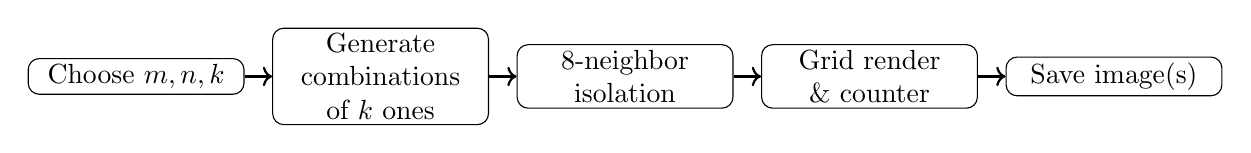
\begin{tikzpicture}[node distance=0.35cm,
                every node/.style={draw, rounded corners, align=center, inner sep=2pt, text width=2.6cm}]
                \node (pick) {Choose $m,n,k$};
                \node (gen)   [right=of pick]  {Generate combinations of $k$ ones};
                \node (check) [right=of gen]   {8-neighbor isolation};
                \node (view)  [right=of check] {Grid render\\\& counter};
                \node (save)  [right=of view]  {Save image(s)};
                \draw[->, thick] (pick) -- (gen);
                \draw[->, thick] (gen)  -- (check);
                \draw[->, thick] (check)-- (view);
                \draw[->, thick] (view) -- (save);
            \end{tikzpicture}}
        \small Alt text: Boxes show the pipeline from selecting parameters to generating, checking, viewing, and saving layouts.
    \end{frame}


    \begin{frame}{Program B in 3 steps}
        \begin{enumerate}\addtolength\itemsep{0.6em}
        \item Systematically place $k$ ones on an $m\times n$ grid.
        \item Check that every zero is isolated in the 8-neighborhood.
        \item Display the matrix and allow navigation or saving to PNG.
        \end{enumerate}
        \small\emph{Advanced note:} Per-matrix validation is $O(mn)$ since there are 8 constant neighbors per cell.
    \end{frame}

    \begin{frame}[fragile]{Program B: tiny Java snippet - full grate check}
        \small
        \begin{tabular}{r l}
            1 & \texttt{private boolean isValidFullGrate(int[][] matrix) \{}\\
            2 & \texttt{        int[] dx = \{-1, 1, 0, 0, -1, -1, 1, 1\};  // Includes diagonal directions}\\
            3 & \texttt{        int[] dy = \{0, 0, -1, 1, -1, 1, -1, 1\};}\\
            4 & \texttt{}\\
            5 & \texttt{        for (int i = 0; i \textless{} rows; i++) \{}\\
            6 & \texttt{            for (int j = 0; j \textless{} cols; j++) \{}\\
            7 & \texttt{                if (matrix[i][j] == 0) \{ // Check if the 0 is isolated}\\
            8 & \texttt{                    for (int d = 0; d \textless{} 8; d++) \{}\\
            9 & \texttt{                        int ni = i + dx[d];}\\
            10 & \texttt{                        int nj = j + dy[d];}\\
            11 & \texttt{                        if (ni \textgreater{}= 0 \&\& ni \textless{} rows \&\& nj \textgreater{}= 0 \&\& nj \textless{} cols \&\& matrix[ni][nj] == 0) \{}\\
            12 & \texttt{                            return false; // Adjacent 0 found (including diagonally), so not a full grate}\\
            13 & \texttt{                        \}}\\
            14 & \texttt{                    \}}\\
            15 & \texttt{                \}}\\
            16 & \texttt{            \}}\\
            17 & \texttt{        \}}\\
            18 & \texttt{        return true;}\\
            19 & \texttt{    \}}\\
        \end{tabular}

        \footnotesize Callouts: (1) Fixed neighbor offsets encode king moves. (2) A zero next to any zero fails the rule.\\
        \footnotesize Caption: See Appendix for full code.
    \end{frame}

    \begin{frame}{Program B: what could go wrong}
        \begin{itemize}\addtolength\itemsep{0.8em}
        \item Large $mn$ and $k$ can make enumeration heavy - keep sizes modest or sample.
        \item Misclicks are not an issue in this viewer - navigation is by buttons with counts shown.
        \item Disk permissions when saving images - handled with standard file chooser and error dialogs.
        \end{itemize}
    \end{frame}

    \begin{frame}{Side-by-side comparison}
        \centering\footnotesize
        \resizebox{\linewidth}{!}{%
            \begin{tabular}{|l|c|c|}
                \hline
                & \textbf{Program A} & \textbf{Program B} \\\hline\hline
                Purpose & Count all valid layouts & Show valid layouts for fixed $k$ \\\hline
                Inputs & $m,n$ & $m,n,k$ \\\hline
                Core idea & DP over compatible masks & Enumerate and filter then render \\\hline
                Output & BigInteger counts by $k$ & Browse and save images \\\hline
                \emph{Advanced concept} & Transfer via $\mathrm{compat}[i][j]$ & 8-neighbor isolation test \\\hline
            \end{tabular}}
    \end{frame}

    \appendix
    \section*{Appendix}
    \begin{frame}{Source files}
        \small
        \begin{itemize}
            \item \texttt{FullGrateCounterGUI.java} - DP counter and GUI.
            \item \texttt{FullGrateVisualizer.java} - enumeration-based viewer with image export.
        \end{itemize}
    \end{frame}

    \frame{\Huge\centering Thank You for Listening!}

    \nocite{oeis}
    \nocite{dickens}

    \begin{frame}{References}
% \bibliographystyle{alpha}
% \bibliography{main}

        \begin{itemize}
            \item Amaca, Edgar (2011). Image from paper titled ``On rational functions with golden ratio as fixed point'' Obtained from: \text{https://www.researchgate.net/figure/A-Pascals-Triangle-Fibonacci-Sequence-Mapping_fig2_228768004}
            \item Dickens, Charles (1861). \textit{Great Expectations}, Chapman \& Hall.
            \item Online Encyclopedia of Integer Sequences (OEIS). Published electronically at https://oeis.org
            \item Darrow, Jr., B. \& Fields, J. (2024). Entry $A365554$. OEIS. Published electronically at https://oeis.org/A365554
            \item Darrow, Jr., B. \& Fields, J. (Accepted). Binary sequences with isolated zeroes.
            \item Lang, Wolfdieter (2002). Entry $A067331$. OEIS. Published electronically at   https://oeis.org/A067331
        \end{itemize}
    \end{frame}





%N.B. This is a really kludgy way of doing a bibliography -Joe
%
%\begin{thebibliography}{99}
%
%\begin{frame}{References}
%\bibitem{BaSt} R.\,F.~Bailey and B.~Stevens,
% Hamilton decompositions of complete $k$-uniform hypergraphs,
% \emph{Discrete Math.} \textbf{310} (2010), 3088--3095.
%
% \bibitem{BrHeMaWa} D.~Bryant, S.~Herke, B.~Maenhaut, and W.~Wannasit,
% Decompositions of complete 3-uniform hypergraphs into small 3-uniform hypergraphs,
% \emph{Australas. J. Combin.} \textbf{60} (2014), 227--254.
%
%    \bibitem{Ke} P.~Keevash,
% The existence of designs, arXiv:1401.3665v2, (2018), 39~pages.
%
%\bibitem{GlKuLoOs1} S.~Glock, D.~K\"uhn, A.~Lo, and D.~Osthus,
% The existence of designs via iterative absorption,
% arXiv:1611.06827v2, (2017), 63~pages.
%
%\bibitem{GlKuLoOs2} S.~Glock, D.~K\"uhn, A.~Lo, and D.~Osthus,
% Hypergraph $F$-designs for arbitrary~$F$,
% arXiv:1706.01800, (2017), 72~pages.
%\end{frame}


%\begin{frame}{References}
%\bibitem{Ha1} H.~Hanani,
% On quadruple systems,
% \emph{Canad. J. Math.}, \textbf{12} (1960), 145--157.
%
%\bibitem{Ha3} H.~Hanani,
% Decomposition of hypergraphs into octahedra,
% Second International Conference on Combinatorial Mathematics (New York, 1978), pp. 260--264, \emph{Ann. New %York Acad. Sci.}, 319, New York Acad. Sci., New York, 1979.
%
%\bibitem{MeRo1} M.~Meszka and A.~Rosa,
% Decomposing complete $3$-uniform hypergraphs into Hamiltonian cycles,
% \emph{Australas. J. Combin.} \textbf{45} (2009), 291--302.
%
%\end{frame}
%\end{thebibliography}

    \section{Conclusion}

    \begin{frame}{A Grate Many Thanks}
        \begin{itemize}
            \setlength\itemsep{1em}
            \item Dr. Joe Fields (research partner, friend, former professor)
            \item N. J. A. Sloane and the OEIS team.
            \item The CCSU Mathematical Sciences Department
            \item Everyone here!
        \end{itemize}
    \end{frame}



\end{document}